\pagestyle{empty}
\cleardoublepage
\pagestyle{fancy}

\chapter{Algoritmo Proposto}\label{cap4}

\section{Introdução}\label{cap4:intro}

Esta seção demonstra detalhes de implementação do algoritmo proposto para o balanceamento de carga dinâmico em aglomerados de GPUs. 

Em uma típica aplicação paralela, os dados da aplicação são divididos entre as threads em um processo chamado decomposição de domínio. As threds entao simultenamente processam parte dos dados. Depois de terminarem, mesclam os resultados processados e terminam a aplicação ou continuam para a próxima fase de computação. A tarefa do algoritmo proposto é determinar o tamanho do bloco de dados atribuído a cada GPU e CPU no sistema. O termo processador significará um única CPU ou GPU.

O algoritmo tem três partes, que são: (1) modelo de desempenho do processador, onde um modelo de execução é determinado durante a execução da aplicação; (2) seleção do tamanho ótimo do bloco, onde baseado no modelo de performance o algoritmo seleciona a melhor distribuição de tamanho de blocos entre os processadores; e (3) o rebalancemaentom onde o algoritmo recalcula o tamanho do bloco ótimo quando a diferença no tempo de execução nos diferentes processadores é maior que um limiar.

Modelo de desempenho do processador. Inicialmente determina-se a função $P_p[x]$, que fornece a velocidade de processamento para um dado bloco de tamanho $x$ no processador $p$. Para construir estas curvas, um bloco de tamanho $initialBlockSize$, definido pelo usuário é alocado para cada processador. Seleciona-se o processador com o menor tempo de processamento $t_f$ e dobra-se o tamnho do bloco para este processador. Para os outros processadores, com o tempo de término $t_i$, selciona-se o tamanho do bloco proporcional a razão $t_i/t_f$.


\begin{figure*}[htb]
	\begin{center}
	\centering
			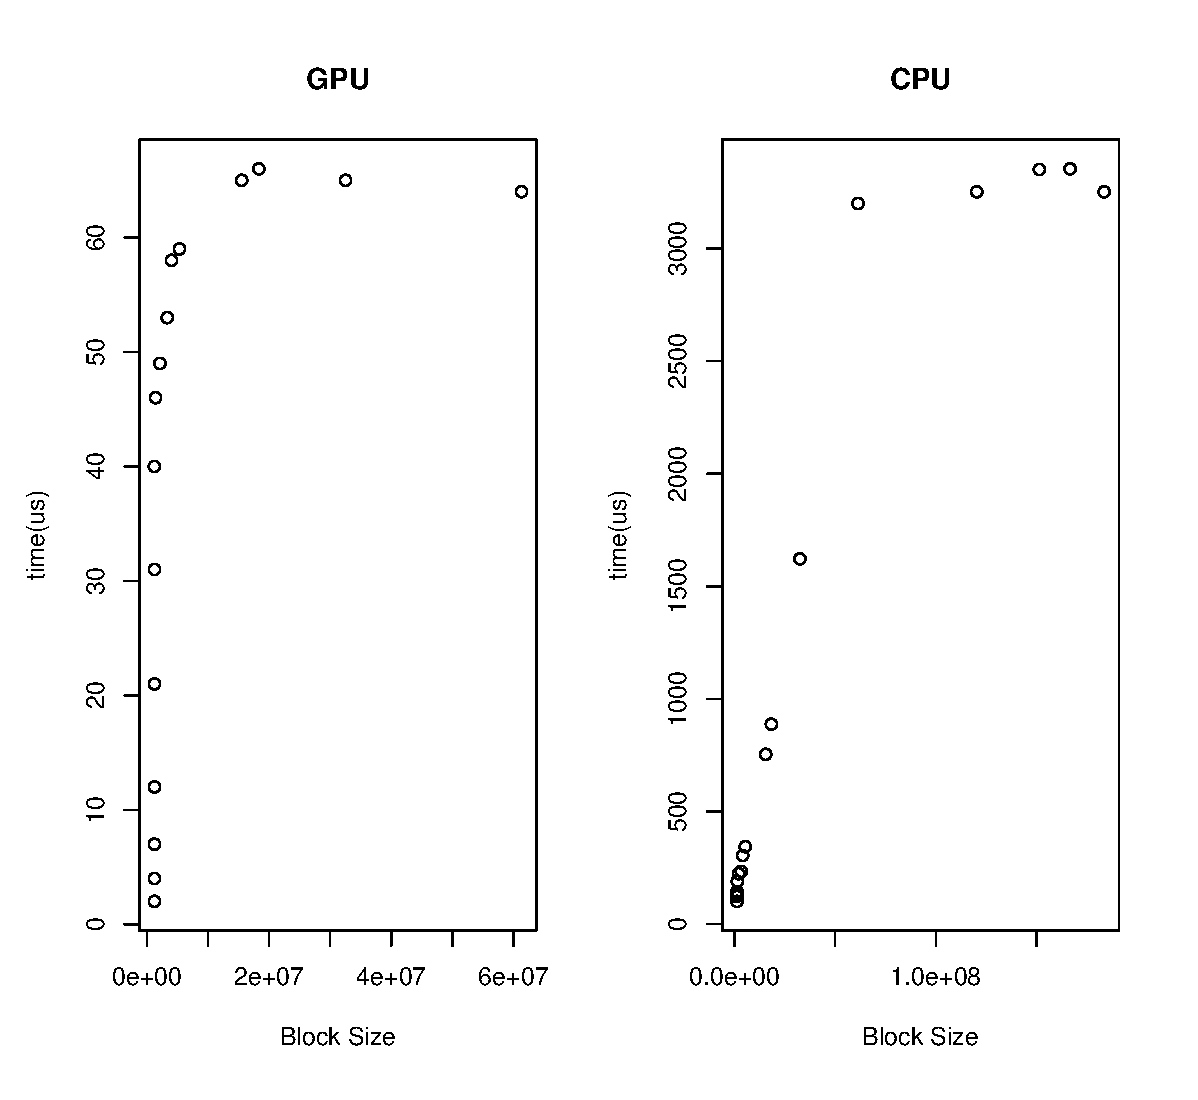
\includegraphics[scale=0.3]{CPUVersusGPU.eps}
	\caption{Curvas para GPU x CPU}
	\label{fig:CPUVersusGPU}
	\end{center}
\end{figure*}


A figura \ref{fig:CPUVersusGPU} mostra um exemplo de media de tempo para uma GPU e uma CPU para diferentes tamanhos de bloco. Pode-se notar que as curvas podem ser aproximadas por funções polinimiais. Nestas curvas encontrou-se as melhores curva que se ajustam através do método dos mínimos quadrados, usando uma função da forma $y= a_1f_1(x) + a_2f_2(x) + a_3f_3(x) + ... + a_nf_n(x)$. A curva é ajustada após a geração de poucos pontos, por exemplo quatro, gerando um modelo de tempo de execução para cada processador.

A figura \ref{fig:CPUVersusGPU} mostra um exemplo d medida de tempo de processamento para uma GPU e uma CPU. pra diferentes tamnhos de bloco em dias aplicações. Pode-se notar que as curvas para aplicação blackscholes pode ser aproximada por funções lineares, enquanto para a multiplicação de matrizes usa-se uma função exponencial. Encontrou-se o melhor ajuste das curvas utilizando o método dos mínimos quadrados:

\begin{equation}
 y = a_{1} f_{1}(x) +  a_{2} f_{2}(x) + ... + a_{n} f_{n}(x) 
\label{eq: least}
\end{equation} 

onde $f_i(x)$ corresponde a um pequeno conjunto de funções de complexidade comum, tais como $x$, $x^2$, $e^x$, $ln x$, etc. 

\begin{algorithm}

\caption{Modelo de desempenho do processador}
\label{algModel}

\begin{algorithmic}		

\STATE \textbf{function}~determineModel()

\STATE $blockSizeList \leftarrow initialBlockSize;$
\WHILE{$fitValues.error \geq 0.5$}
		\STATE $finishTimes$ = executeTasks($blockSizeList$);
                \STATE synchronize();
	        \STATE $blockSizeList$ = evaluateNextBlockSizes($finishTimes$);
		\STATE $fitValues$ = determineCurveProcessor();
\ENDWHILE

return $fitValues$;

\end{algorithmic}
\end{algorithm}

Estes passos são mostrados no algoritmo \ref{algModel}. A variável $blockListSize$ contem o tamanhos dos blocos atribuídos a cada processador e é inicializada com $initialBlocoSize$, que é definida  pelo usuário. A variável $fitValues$ contem o resultado do ajuste por mínimos quadrados, incluindo o erro no ajuste, que é incializado como $+\infty$.

No laço inicia, enquano o erro é maior que um valor pré definido, a função envia um pedaço de dados para cada processador e obtem o tempo que demorou para realizar o processament em cada processador. Depois de esperar, que todos os processadores terminem, é determinado o tamnho do bloco para a próxima iteração, baseado no tempo de término de cada processador. Por fim, o algoritmo tenta ajustar um modelo de curva para cada processador e recebe o resultado do ajuste.

Seleção do tamanho de bloco ótimo: O algoritmo determina o tamanho do bloco ótimo para cada processador com o objetivo de minimizar o  tempo total da aplicação. Considere que existem $n$ processadores e o tamanho da entrada seja $Z$. O algoritmo atribui um pedaço de dados de tamnho $x^g$ para cada processador $g= 1,..., n$, correpondendo a uma fração dos dados de entrada, tal que $\sum_{g=1}^n x^g = Z$. Denota-se como $E^g(x^g)$ o tempo de execução da tarefa $E$ no processador $g$, para cada entrada de tamanho $x^g$. Para distribuir o trabalho entre os processadores, encontra-se um conjunto de valores:

\begin{equation}
	X = \{ x^g \in \mathbb{R}:[0,1] / \sum_{g=1}^n x^g = Z \}
	\label{eq: totalResultado}
\end{equation}

que minimiza $E_1(x_1)$ enquanto satisfaz a restrição:

\begin{equation}
	E_{1} = E_{2} = ...= E_{n}
	\label{eq: Restricao}
\end{equation}
 
que representa que todos os processadores gastariam uma mesma quantidade de tempo realizando o processamento. Para determinar o conjunto de valores de $x$, resolve-se o sistema de equações das curvas ajustadas para todos os processadores, dados por:

\begin{equation}
	\left\lbrace
	\begin{array}{ll}
		\displaystyle E_{1} = f(x_{1})  \\
		\displaystyle E_{2} = f(x_{2})   \\
		\displaystyle E_{n} = f(x_{n}) 
		\label{eq: system}
	\end{array}
	\right.
\end{equation}

O sistema de equações é resolvido aplicando interior \emph{point line search filter method}. O algoritmo busca minimozar as funções no espaço de busca. Ele alcança uma solução ótima percorrendo o interior de uma solução viável. Determinar o valor de $x$ tal que o tempo é mínimo.

Rebalanceamento: Depois de resolver o sistema de equações o escalonador mantem enviando tarefas de tamanho $x_i$ para cada processador $i$, logo que o processador termina a tarefa anterior. Também monitora o tempo de término de cada tarefa. Se a diferença no tempo de término entre $x_i$ e $x_j$ de qualquer duas tarefas $i$ e $j$ for maior que um limiar, o processo de balanceamento é reexecutado. Neste caso, o algoritmo aplica o modelo de desempenho e a rotina de determinação do tamanho do bloco ótimo novamente. O escalonador então sincroniza as tarefas e inicia usando o novo valor de $x_i$. O limiar precisa ser determinado empiricamente através de alguns testes. Se o limiar é um valor muito pequeno, ocorre balanceamentos desnecessários, que aumentará o tempo total da aplicação. Se o limiar é muito grande balanceamento necessários podem não ocorrer, o que pode fazer com que threads fiquem ociosas.

\begin{figure}[!t]
	\centering
			\includegraphics[scale=0.24]{DiagramaArtigo.png}
	\caption{Execução das Threads com limiar}
	\label{fig:Diagrama}
\end{figure}

A figura \ref{fig:Diagrama} apresenta um diagrama de execucão para quatro threads e uma thread desbalanceada. As caixas representam os limiares, as linas as threads e os círculos o desbalanceamento. As threads iniciam sincronizadas, recebem carga, mas em um segundo passo uma thread leva mais tempo que o valor de limiar, isto causa o desbalanceamento. Detectado o desbalanceamento, todas as threads são sincronizadas, e as partes são recalculadas para cada thread, fazendo com que as threads voltem ao estado sincronizado.



\begin{algorithm}

\caption{Complete dynamic algorithm}
\label{alg1}

\begin{algorithmic}		

\STATE \textbf{function} dynamic()

\STATE $fitValues$ = determineModel()
\STATE $X$ = solveEquationSystem($fitValues$);

\WHILE{there is data}

	\STATE $finishTimes$ = executeTasks($X$);
	\IF {$ $maxDifference($finishTimes$)$ \geq threshold$}
		\STATE $fitValues$ = determineCurveProcessor();
                \STATE $X$ = solveEquationSystem($fitValues$);
                \STATE synchronize();
    	\ENDIF
\ENDWHILE

\end{algorithmic}
\end{algorithm}

Algoritmo Completo: Algoritmo \ref{alg1} apresenta o pseudocódigo do algoritmo de escalonamento. A função $determineModel$ mostrada no algoritmo \ref{algModel} retorna o modelo de desempenho para cada processador. Então resolve o sistema de equações para determinar a melhor distribuição de pedaços de dados para cada processador.

O laço inicial repete enquanto há dados ainda para serem processados. É distribuído pedaços de dados para cada processador do sistema, obtendo o tempo de término para cada execução de tarefa. É checado se a diferença maxima entre o término das tarefas está acima de um limar, obtido empiricamente. Se o limiar é alcançado, o algorimto ajusta um novo modelo de curvas e resolve o sistema de equações para estas novas curvas para determinar uma nova distribuição de tamanhos pedaços de dados.

 


\section{IPOPT}\label{cap4:ipopt}

IPOPT (Interior Point Optimizer) é um pacote de software aberto para otimização não linear. IPOPT pode resolver problemas de programação não-linear da seguinte forma:
	


onde x $\in$ a $\Re ^ n$ são as variaveis de otimização, $f : R^n em R$ é a função objetivo, e $g: R^n$ em $R^M$ são as restrições não lineares. A função $f(x)$ e $g(x)$ podem ser linear ou não linear.  

Para resolver um problema de otimização precisa-se criar um IpoptProblem com a função CreateIpoptProblem, que posteriormente precisa ser passado para a função IpoptSolve. O IpoptProblem criado por CreateIpoptProblem contem as dimensões do problema, as variaveis e os limites das restrições.








